% RLVIB --- FINAL deck.  Build:  cd paper && tectonic final.tex
%
% Merge of paper/slides.tex (weekly, math-heavy) and paper/phd_talk.tex (intro, schema-heavy),
% restricted to numbers that are GROUNDED:
%   (a) measured by us   -> the source runs/*.json is named in a "% src:" comment, or
%   (b) reported by a cited paper -> the arXiv id is named in the row/comment.
% Nothing invented appears in this file. Content dropped for lack of evidence:
%   3-seed statistics, likelihood-shift values, VIB-placement ablation, beta_kl sweep,
%   VIB-ingredient ablation, data-scaling curve, swap-video / shift-DPO / MiniCPM-trained /
%   cross-attention results (those runs are in flight; add rows when their JSONs land).
\documentclass[aspectratio=169,11pt]{beamer}
\usetheme{default}
\usecolortheme{seahorse}
\setbeamertemplate{navigation symbols}{}
\setbeamertemplate{footline}[frame number]
\setbeamertemplate{itemize items}[circle]
\setbeamertemplate{blocks}[rounded][shadow=false]
\setbeamerfont{frametitle}{size=\large,series=\bfseries}
\setbeamercolor{frametitle}{fg=blue!45!black}
\usepackage{tikz}
\usetikzlibrary{positioning,arrows.meta}
\usepackage{booktabs}
\usepackage{amsmath,amssymb}
\graphicspath{{figures/}}
\definecolor{frz}{RGB}{40,95,175}     % frozen
\definecolor{trn}{RGB}{210,120,20}    % trained
\newcommand{\fillin}[1]{\textcolor{red!70!black}{[#1]}}
\newcommand{\figslot}[2]{\IfFileExists{figures/#1}%
  {\includegraphics[width=#2]{figures/#1}}%
  {\fbox{\parbox[c][2.6cm][c]{#2}{\centering\tiny\ttfamily\detokenize{figures/#1}}}}}
\newcommand{\frm}[1]{\IfFileExists{figures/#1}{\includegraphics[height=15mm]{figures/#1}}%
  {\fcolorbox{gray}{gray!12}{\parbox[c][14mm][c]{20mm}{\centering\tiny\ttfamily\detokenize{#1}}}}}
\newcommand{\frmrow}[1]{\frm{#1_1.jpg}\hspace{1pt}\frm{#1_2.jpg}\hspace{1pt}\frm{#1_3.jpg}}
\newcommand{\exrow}[5]{%
  \begin{tikzpicture}[font=\scriptsize,>={Latex[length=1.6mm]}]
    \node[draw=black!30,rounded corners=2pt,inner sep=1.5pt] (im) {\frmrow{#1}};
    \node[anchor=west,align=left,text width=58mm,inner sep=0pt] (c) at ([xshift=7mm]im.east)
      {#2\\[2pt]\emph{#3}};
    \draw[->,black!45] (im.east) -- (c.west);
    \node[draw=red!60!black,fill=red!8,rounded corners=2pt,inner sep=2.5pt,anchor=north west]
      (b) at ([yshift=-3pt]c.south west) {\color{red!72!black}base: #4 $\boldsymbol{\times}$};
    \node[draw=green!45!black,fill=green!12,rounded corners=2pt,inner sep=2.5pt,anchor=west]
      (o) at ([xshift=3mm]b.east) {\color{green!48!black}ours: #5 $\boldsymbol{\checkmark}$};
  \end{tikzpicture}}

\title{\textbf{Making Frozen Audio--Visual LLMs Listen}}
\subtitle{Audio grounding via tiny adapters, anchored preference optimization, and honest evaluation}
\author{Souleiman Sbai}
\institute{Research internship --- final presentation\\[2pt]
  \small Host lab: \fillin{laboratory} \quad$\cdot$\quad Supervisor: \fillin{supervisor}}
\date{\today}

\begin{document}

% ============ Title ============
{\setbeamertemplate{footline}{}
\begin{frame}
\titlepage
\vspace{-1.2em}
\begin{block}{}
\small \textbf{The problem in one line:} audio-visual LLMs answer sound questions from the
\emph{picture}. \textbf{This internship:} a tiny module that makes a \emph{frozen} model listen ---
without retraining it, and measured honestly.
\end{block}
\end{frame}}

% ================================================================
% ================================================================

\begin{frame}{What is an audio--visual LLM?}
\centering
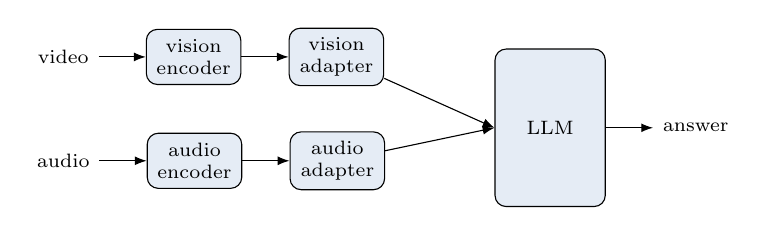
\begin{tikzpicture}[font=\scriptsize,>={Latex[length=1.5mm]},node distance=3.5mm and 6mm,
  enc/.style={draw,rounded corners,fill=frz!12,minimum width=12mm,minimum height=7mm,align=center},
  llm/.style={draw,rounded corners,fill=frz!12,minimum width=14mm,minimum height=20mm,align=center},
  io/.style={align=center}]
  \node[io] (vin) {video};
  \node[enc,right=of vin] (venc) {vision\\encoder};
  \node[enc,right=of venc] (vproj) {vision\\adapter};
  \node[io,below=9mm of vin] (ain) {audio};
  \node[enc,right=of ain] (aenc) {audio\\encoder};
  \node[enc,right=of aenc] (aproj) {audio\\adapter};
  \node[llm,right=14mm of vproj,yshift=-9mm] (llm) {LLM};
  \node[io,right=of llm] (ans) {answer};
  \draw[->] (vin)--(venc); \draw[->] (venc)--(vproj); \draw[->] (vproj)--(llm.west);
  \draw[->] (ain)--(aenc); \draw[->] (aenc)--(aproj); \draw[->] (aproj)--(llm.west);
  \draw[->] (llm.east)--(ans);
\end{tikzpicture}
\vspace{0.5em}
\begin{itemize}\small
\item Each modality is encoded into \textbf{tokens} (audio $\sim$25/s; video sampled at
\textbf{2\,fps} in all our Qwen3-Omni runs), projected by a small \emph{adapter} into the LLM's
embedding space, and concatenated with the question.
\item The LLM answers over the \textbf{mixed token sequence} --- text, audio and vision compete
for its attention.
\item Test beds: Qwen3-Omni (30B MoE), Qwen2.5-Omni (7B), VideoLLaMA2, MiniCPM-O 2.6.
\end{itemize}
\end{frame}

\begin{frame}{The failure we study: cross-modal hallucination}
\centering
\begin{tabular}{@{}c@{}}
\exrow{avh_a2v}{\textbf{audio $\to$ video} {\scriptsize(the sound makes it ``see'')}}{hear: harsh grinding, like a power tool. ``Is a power tool visible?'' --- no.}{``Yes''}{``No''} \\[2.5mm]
\exrow{avh_v2a}{\textbf{video $\to$ audio} {\scriptsize(the image makes it ``hear'')}}{see: a parrot on a shoulder; the clip is silent. ``Is the bird making sound?''}{``Yes''}{``No''}
\end{tabular}
\vfill
\small The model \textbf{over-trusts what it sees} and \textbf{under-uses what it hears}: it sees
objects the audio suggests (top), and invents sounds the image implies (bottom).
\end{frame}

\begin{frame}{Not a quirk of our setup: models lean on vision, not audio}
\begin{itemize}\footnotesize\setlength\itemsep{3pt}
\item \textbf{AVHBench} (Sung-Bin et al., ICLR'25): every AV-LLM tested invents sounds from sights
and objects from sounds --- cross-modal hallucination is the norm.
\item \textbf{CMM} (Leng et al., 2024): traces it to \emph{over-reliance on unimodal priors} ---
audio is the weakest, most-overridden channel.
\item \textbf{``When vision speaks for sound''} (Wen et al., 2026): a \emph{Clever Hans} effect ---
models answer sound questions from \textbf{visual priors}.
\item Proposed fixes: contrastive decoding (MAD), modality-decoupled DPO (MoD-DPO), full-model
re-alignment --- \textbf{none keeps the backbone frozen}.
\end{itemize}
\vfill
\centering
{\footnotesize Wen et al.'s audio interventions on \textbf{Qwen3-Omni} --- \emph{our} backbone (accuracy, \%):}\\[3pt]
\footnotesize
\begin{tabular}{l cc l}
\toprule
probe & original & intervened & intervention \\
\midrule
audio existence   & 95.1  & \textcolor{red!70!black}{\textbf{0.0}}  & \emph{Mute}: silence the track \\
temporal sync     & 100.0 & \textcolor{red!70!black}{\textbf{1.4}}  & \emph{Shift}: audio moved $\pm 2$\,s \\
sound consistency & 75.4  & \textcolor{red!70!black}{\textbf{37.3}} & \emph{Swap}: another clip's audio \\
\bottomrule
\end{tabular}\\[3pt]
{\scriptsize Reported, arXiv:2605.16403 Tab.~1. Mute the audio and the model still ``hears'' what
the pixels imply.}
\end{frame}

\begin{frame}{Objective and contributions}
\begin{center}\large\itshape
Can we make a \textbf{frozen} AV-LLM ground its answers in what it hears,\\[2pt]
by training something \textbf{tiny} bolted onto it?
\end{center}
\vspace{0.3em}
\begin{itemize}\small
\item[\textbf{C1}] A \textbf{variational-bottleneck adapter} ($<$0.5\% of params), \emph{exactly
identity at initialization}.
\item[\textbf{C2}] An \textbf{anchored swap-DPO} objective that fixes the collapse naïve preference
optimization falls into --- one engine, two safety rails.
\item[\textbf{C3}] A \textbf{prompt-aware (FiLM)} variant, and attention evidence that it grounds by
a \emph{faithful} mechanism.
\item[\textbf{C4}] An \textbf{honest harness}: pinned decoding, held-out selection, paired
statistics, three capability guards, four backbones.
\item[\textbf{C5}] A \textbf{temporal extension} --- design, data and benchmark for \emph{when},
with the baseline measured.
\end{itemize}
\end{frame}

% ================================================================
% ================================================================

\begin{frame}{Benchmark I --- AVHBench (the target)}
\begin{columns}[T]
\begin{column}{0.5\textwidth}
\footnotesize
\setlength{\tabcolsep}{4pt}
\begin{tabular}{@{}lrrr@{}}
\toprule
Judgment task & QnA & yes & no \\
\midrule
A$\to$V (audio$\to$video) & 1,136 & 568 & 568 \\
V$\to$A (video$\to$audio) & 2,290 & 1,145 & 1,145 \\
A--V Matching             & 1,876 & 938 & 938 \\
\midrule
\textbf{Total}            & \textbf{5,302} & 2,651 & 2,651 \\
\bottomrule
\end{tabular}
\par\vspace{0.4em}
{\scriptsize 2,136 everyday videos; yes/no \textbf{exactly balanced}, so a constant answer scores
50\% --- accuracy is honest.}
\end{column}
\begin{column}{0.5\textwidth}\scriptsize
\textbf{The three yes/no tasks}
\begin{itemize}
\item \textbf{A$\to$V}: ``is the queried object \emph{visible}?'' --- the \emph{heard} event tempts a
false yes.
\item \textbf{V$\to$A}: ``is the queried sound \emph{audible}?'' --- the \emph{seen} event tempts a
false yes. \textbf{Our audio-grounding probe.}
\item \textbf{A--V Matching}: ``do audio and video \emph{match}?'' --- needs real cross-modal
integration.
\end{itemize}
\end{column}
\end{columns}
\end{frame}

\begin{frame}{Benchmark II --- CMM (the capability guard)}
\centering
{\footnotesize \textbf{1,200 samples $\times$ 2 probes $=$ 2,400 questions}: one \emph{present} object
(gold ``yes''), one \emph{absent} (gold ``no'') per sample.}
\vspace{0.5em}
\[
\mathbf{PA}=\frac{\#\,\text{correct ``yes''}}{\#\,\text{ground-truth ``yes''}}
\qquad\qquad
\mathbf{HR}=\frac{\#\,\text{correct ``no''}}{\#\,\text{ground-truth ``no''}}
\]
\begin{center}
\setbeamercolor{block body}{bg=red!6}
\begin{block}{Why you must watch BOTH numbers}
\centering\small A model that answers ``no'' to everything gets \textbf{HR $=$ 1.0} (never
hallucinates!) but \textbf{PA $=$ 0} (perceives nothing). Any hallucination fix must be checked
against the trap of just \emph{saying no more often}.
\end{block}
\end{center}
\vfill
{\footnotesize This trap is not hypothetical --- it is exactly what our first training run did.}
\end{frame}

\begin{frame}{Protocol: the harness is pinned}
\begin{itemize}\small
\item \textbf{Frame rate fixed at 2\,fps} for Qwen3-Omni (1\,fps for the 7B backbones), \emph{in
code}, across the selection grid \emph{and} the final eval --- below 2\,fps Qwen3 starves and drifts
to a yes-bias.
\item \textbf{The harness is a lever}: changing only the answer-format suffix moved one score by
\textbf{$+11$ points} (V$\to$A $69.0 \to 80.3$) on \emph{identical weights}. So prompts, suffix and
decoding are frozen and logged. \hfill{\scriptsize src: sysfull vs full eval JSONs}
\item \textbf{Selection on a validation half, report on the disjoint rest} --- never select on the
test set. Our first ``best'' checkpoint did not survive this.
\item \textbf{Paired statistics}: same items for both models, McNemar $+$ bootstrap CI.
\item \textbf{Leakage check}: training clips $\cap$ benchmark clips $= \varnothing$, scripted.
\end{itemize}
\vfill
\begin{center}
\setbeamercolor{block body}{bg=blue!6}
\begin{block}{}
\centering\small A single number is worth only as much as the harness under it.
\end{block}
\end{center}
\end{frame}

% ================================================================
% ================================================================

\begin{frame}{Background: the Variational Information Bottleneck}
{\small \textbf{Idea} (Tishby et al., 2000): learn a compressed code $Z$ of the input $X$ that keeps
\emph{only} what predicts the target $Y$ --- and forgets the rest.}
\vspace{-0.2em}
\[
\max_{q(z|x)}\ \underbrace{I(Z;Y)}_{\text{keep what predicts }Y}\ -\ \beta\,\underbrace{I(Z;X)}_{\text{forget the rest of }X}
\]
\vspace{-0.5em}
\begin{itemize}\small
\item Both mutual informations are intractable $\Rightarrow$ \textbf{variational bounds} (Alemi et
al., ICLR'17): compression $I(Z;X)\le \mathbb E_x\,\mathrm{KL}\!\big(q(z|x)\,\|\,\mathcal N(0,I)\big)$
--- the ``\textbf{rate}''; relevance $=$ the ordinary prediction loss.
\item \textbf{Stochastic encoder} (reparameterization): $z=\mu(x)+\sigma(x)\odot\epsilon$,
$\epsilon\sim\mathcal N(0,I)$ --- gradients flow, and the injected noise gives free exploration.
\item $\beta$ trades compression against accuracy --- it is our loss's $\beta_{kl}$.
\end{itemize}
\end{frame}

\begin{frame}{Our module: a variational bottleneck per modality stream}
\centering
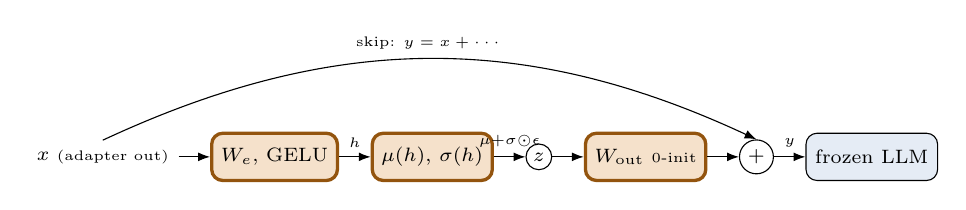
\begin{tikzpicture}[font=\scriptsize,>={Latex[length=1.5mm]},node distance=2mm and 4mm,
  trn/.style={draw,very thick,rounded corners,fill=trn!22,draw=trn!70!black,minimum height=6mm,align=center},
  frzs/.style={draw,rounded corners,fill=frz!12,minimum height=6mm,align=center},
  op/.style={draw,circle,inner sep=1.5pt},
  io/.style={align=center}]
  \node[io] (x) {$x$ {\tiny(adapter out)}};
  \node[trn,right=of x] (enc) {$W_e$, GELU};
  \node[trn,right=of enc] (ms) {$\mu(h),\,\sigma(h)$};
  \node[op,right=of ms] (z) {$z$};
  \node[trn,right=of z] (wout) {$W_{\text{out}}$ {\tiny 0-init}};
  \node[op,right=of wout] (add) {$+$};
  \node[frzs,right=of add] (llm) {frozen LLM};
  \draw[->] (x)--(enc); \draw[->] (enc)--node[above]{\tiny $h$}(ms);
  \draw[->] (ms)--node[above]{\tiny $\mu{+}\sigma{\odot}\epsilon$}(z);
  \draw[->] (z)--(wout); \draw[->] (wout)--(add);
  \draw[->] (add)--node[above]{\tiny $y$}(llm);
  \draw[->] (x.north) to[out=25,in=155] node[above,pos=0.5]{\tiny skip: $y=x+\cdots$} (add.north);
\end{tikzpicture}
\vspace{0.4em}
\[ z=\mu(x)+\sigma(x)\odot\epsilon \qquad y = x + W_{\text{out}}\,z \qquad W_{\text{out}}\stackrel{\text{init}}{=}0 \]
\begin{itemize}\small
\item \textbf{Zero-init} $\Rightarrow$ $y=x$ at the start: attaching it changes \emph{nothing} until trained.
\item A \texttt{bypass} switch gives the \textbf{exact frozen base for free} --- the DPO reference
model, at no memory cost.
\item One per modality (audio, vision); together $<$0.5\% of the backbone's parameters.
\end{itemize}
\end{frame}

\begin{frame}{The training signal: manufacture an audio--vision conflict}
\centering
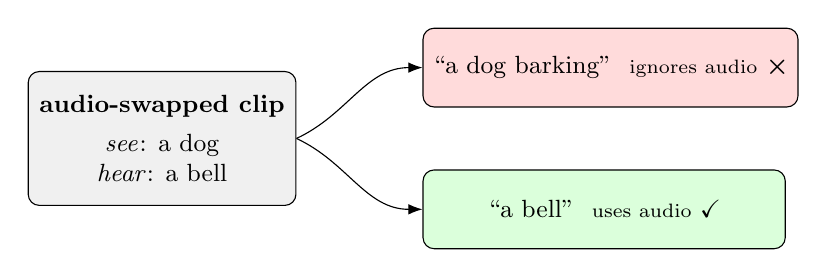
\begin{tikzpicture}[font=\small,>={Latex[length=1.8mm]},
  clip/.style={draw,rounded corners,fill=gray!12,align=center,minimum width=34mm,minimum height=17mm},
  good/.style={draw,rounded corners,fill=green!14,align=center,minimum width=46mm,minimum height=10mm},
  bad/.style={draw,rounded corners,fill=red!14,align=center,minimum width=46mm,minimum height=10mm}]
  \node[clip] (clip) {\textbf{audio-swapped clip}\\[1mm]\emph{see}: a dog\\\emph{hear}: a bell};
  \node[bad,right=16mm of clip,yshift=9mm] (bad) {``a dog barking'' \ {\scriptsize ignores audio} $\boldsymbol{\times}$};
  \node[good,right=16mm of clip,yshift=-9mm] (good) {``a bell'' \ {\scriptsize uses audio} $\boldsymbol{\checkmark}$};
  \draw[->] (clip.east) to[out=25,in=180] (bad.west);
  \draw[->] (clip.east) to[out=-25,in=180] (good.west);
\end{tikzpicture}
\vspace{0.4em}
\par
\exrow{as_flute}{\emph{see} flute, \textbf{hear (overlaid) train horn}}{``Which event do you hear?''}{``flute''}{``train horn''}
\vfill
\small Swap a clip's audio track (one \texttt{ffmpeg} call) $\Rightarrow$ seen $\neq$ heard.
Preferring the \textbf{heard} answer on the \emph{same} clip is only possible by \textbf{using the
audio}.
\end{frame}

\begin{frame}{First attempt: na\"ive preference optimization collapses}
\vspace{-0.2em}
\[
\mathcal L_{\text{DPO}}
=-\log\sigma^{\textcolor{trn}{*}}\Big(\beta^{\textcolor{trn}{**}}\big[\underbrace{(c_p-c_r)}_{\text{chosen: gain over base}}
-\underbrace{(r_p-r_r)}_{\text{rejected: gain over base}}\big]\Big)
\]
{\tiny \textcolor{trn}{$^{*}$}\,$\sigma=$ logistic sigmoid (\emph{not} the encoder's std-dev $\sigma(x)$).\quad
\textcolor{trn}{$^{**}$}\,$\beta=$ DPO temperature ($0.1$; \emph{not} the VIB rate $\beta_{kl}$).}
\vspace{2pt}
{\scriptsize $c,r$ $=$ log-probs of the chosen (heard) / rejected (seen) answer; subscript $p$ $=$
adapter on, $r$ $=$ adapter bypassed $=$ the frozen base --- our reference model, for free.}
\vspace{0.2em}
\begin{itemize}\small
\item Train with this, the \textbf{standard DPO loss}, on the swap pairs $\Rightarrow$ perception
accuracy \textbf{0.95 $\to$ 0.10}; the model answers ``no'' to \emph{everything}.
\item The loss sees \textbf{only the margin} --- it is satisfied even when \emph{both} answers'
probabilities fall and the mass drains onto a constant ``no'' (\emph{likelihood displacement}).
\item And recall the CMM trap: all-``no'' looks \textbf{perfect} on hallucination metrics.
\end{itemize}
\vfill
\begin{center}
\setbeamercolor{block body}{bg=red!8}
\begin{block}{}
\centering\small First lesson: \textbf{a hallucination metric alone cannot be your training target.}
\end{block}
\end{center}
\end{frame}

\begin{frame}{The fix: one engine, two safety rails}
\vspace{-0.3em}
\begin{align*}
\mathcal L =\ & \underbrace{-\log\sigma(\beta[(c_p{-}c_r){-}(r_p{-}r_r)])}_{\text{\textbf{engine}: prefer the heard answer}}
 \;+\; \lambda_a\,\underbrace{\big({-}\log\sigma(\beta(c_p{-}c_r){-}\delta)\big)}_{\text{\textcolor{trn}{\textbf{rail 1}: chosen $\ge$ base $\Rightarrow$ PA}}} \\[2pt]
 &+\; \lambda_{kl}\,\underbrace{\mathrm{KL}\!\big(p_{\text{base}}\,\|\,p_\theta\big)}_{\text{\textcolor{trn}{\textbf{rail 2}: normal inputs unchanged $\Rightarrow$ HR}}}
 \;+\; \beta_{kl}\,\mathrm{KL}_{\text{VIB}}
\end{align*}
\vspace{-0.3em}
\begin{itemize}\small
\item \textbf{Rail 1} forbids the collapse route: the chosen answer may never sink below its base
probability (the mDPO-style anchor).
\item \textbf{Rail 2} pins behavior on ordinary (non-swap) inputs, so capability is preserved.
\item Result: answering ``no'' to everything now \emph{fires both rails} --- the only way to lower
the engine's loss is to actually use the audio.
\end{itemize}
\end{frame}

\begin{frame}{FiLM: let the \emph{question} steer the adapter}
\centering
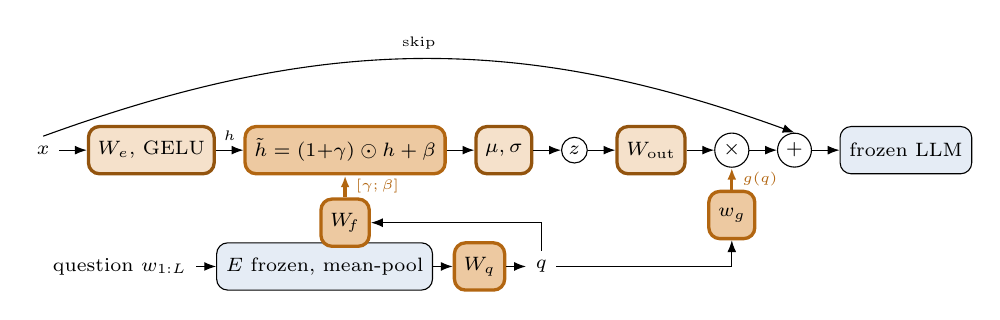
\begin{tikzpicture}[font=\scriptsize,>={Latex[length=1.5mm]},node distance=2mm and 3.5mm,
  trn/.style={draw,very thick,rounded corners,fill=trn!22,draw=trn!70!black,minimum height=6mm,align=center},
  new/.style={draw,very thick,rounded corners,fill=trn!40,draw=trn!85!black,minimum height=6mm,align=center},
  frzs/.style={draw,rounded corners,fill=frz!12,minimum height=6mm,align=center},
  op/.style={draw,circle,inner sep=1.5pt},
  io/.style={align=center}]
  \node[io] (x) {$x$};
  \node[trn,right=of x] (enc) {$W_e$, GELU};
  \node[new,right=of enc] (film) {$\tilde h=(1{+}\gamma)\odot h+\beta$};
  \node[trn,right=of film] (ms) {$\mu,\sigma$};
  \node[op,right=of ms] (z) {$z$};
  \node[trn,right=of z] (wout) {$W_{\text{out}}$};
  \node[op,right=of wout] (mult) {$\times$};
  \node[op,right=of mult] (add) {$+$};
  \node[frzs,right=of add] (llm) {frozen LLM};
  \draw[->] (x)--(enc); \draw[->] (enc)--node[above]{\tiny $h$}(film);
  \draw[->] (film)--(ms); \draw[->] (ms)--(z);
  \draw[->] (z)--(wout); \draw[->] (wout)--(mult); \draw[->] (mult)--(add);
  \draw[->] (add)--(llm);
  \draw[->] (x.north) to[out=20,in=160] node[above,pos=0.5]{\tiny skip} (add.north);
  \node[io,below=13mm of x,anchor=west] (w) {question $w_{1:L}$};
  \node[frzs,right=2.5mm of w] (embed) {$E$ frozen, mean-pool};
  \node[new,right=2.5mm of embed] (wq) {$W_q$};
  \node[io,right=2.5mm of wq] (qv) {$q$};
  \node[new] (wf) at ([yshift=-6mm]film.south) {$W_{\!f}$};
  \node[new] (wg) at ([yshift=-6mm]mult.south) {$w_g$};
  \draw[->] (w)--(embed); \draw[->] (embed)--(wq); \draw[->] (wq)--(qv);
  \draw[->] (qv.north) |- (wf.east);
  \draw[->] (qv.east) -| (wg.south);
  \draw[->,trn!85!black,very thick] (wf.north)--node[right]{\tiny $[\gamma;\beta]$}(film.south);
  \draw[->,trn!85!black,very thick] (wg.north)--node[right]{\tiny $g(q)$}(mult.south);
\end{tikzpicture}
\vspace{0.4em}
\begin{columns}[T]
\begin{column}{0.5\textwidth}
{\scriptsize \textcolor{trn}{\textbf{Main path}} {\normalfont(the plain VIB)}}
\begin{itemize}\scriptsize\setlength\itemsep{1pt}
\item $W_e$: encoder --- lifts token $x$ into hidden $h$
\item $\mu,\sigma$: latent heads --- $z=\mu+\sigma\odot\epsilon$
\item $W_{\text{out}}$: output, \textbf{zero-init}
\end{itemize}
\end{column}
\begin{column}{0.5\textwidth}
{\scriptsize \textcolor{trn}{\textbf{Question path}} {\normalfont(new in FiLM)}}
\begin{itemize}\scriptsize\setlength\itemsep{1pt}
\item $W_q$: pools frozen embeddings $E$ into $q$
\item $W_{\!f}$: $q\mapsto[\gamma;\beta]$ --- per-feature \textbf{scale} \& \textbf{shift}
\item $w_g$: $q\mapsto g(q)\!\in\!(0,1)$ --- \textbf{volume knob}
\end{itemize}
\end{column}
\end{columns}
\vspace{2pt}
{\scriptsize \textcolor{frz}{\textbf{Blue} $=$ frozen}. $\gamma,\beta$ are FiLM's scale/shift (Perez
et al., 2018), \emph{not} the loss's $\beta$ or $\beta_{kl}$. Zero-init $\Rightarrow$ identity at start.}
\end{frame}

\begin{frame}{Why the question \emph{must} be used (a 3-row argument)}
{\small One swapped clip: \emph{see} a dog, \emph{hear} a bell. Ask ``what do you HEAR?'' (answer:
bell) and ``what do you SEE?'' (answer: dog). \textbf{Same pixels, same waveform --- only the
question differs.} Loss per question $=-\log\sigma(m)$: $m{=}{+}2\!\to\!0.13$,
$m{=}0\!\to\!0.69$, $m{=}{-}2\!\to\!2.13$.}
\vspace{0.4em}
\centering
\renewcommand{\arraystretch}{1.15}
\footnotesize
\begin{tabular}{l l cc c}
\toprule
adapter & answers (HEAR / SEE) & HEAR loss & SEE loss & total \\
\midrule
can't read $q$, commits to ``bell'' & ``bell'' / ``bell'' & $0.13$ & $2.13$ & $2.26$ \\
can't read $q$, hedges 50/50        & --- & $0.69$ & $0.69$ & $\mathbf{1.39}$ (floor) \\
\textbf{reads $q$}                  & ``bell'' / ``dog''  & $0.13$ & $0.13$ & $\mathbf{0.26\to 0}$ \\
\bottomrule
\end{tabular}
\vspace{0.5em}
\par
{\small Question-blind adapters are stuck at $\ge 2\log 2\approx 1.39$ per pair; question-aware ones
reach $0$ $\Rightarrow$ the \emph{data construction} forces the adapter to use the question. This is
an argument about the objective, not a measurement.}
\end{frame}

% ================================================================
% ================================================================

\begin{frame}{Main result (Qwen3-Omni, full benchmarks)}
\centering
\renewcommand{\arraystretch}{1.2}
\footnotesize
\begin{tabular}{l cccc ccc}
\toprule
& \multicolumn{4}{c}{AVHBench (n$=$5302)} & \multicolumn{3}{c}{CMM (n$=$2400)} \\
\cmidrule(lr){2-5}\cmidrule(lr){6-8}
 & $A\!\to\!V$ & $V\!\to\!A$ & AV-m & overall & PA & HR & overall \\
\midrule
Gemini {\tiny(closed)} & 0.850 & 0.747 & 0.603 & 0.718 & 0.907 & 0.628 & 0.768 \\
GPT-4o {\tiny(closed)} & 0.846 & 0.510 & 0.501 & 0.579 & 0.359 & 0.892 & 0.626 \\
\midrule
frozen base            & \textbf{0.838} & 0.812 & 0.653 & 0.761 & \textbf{0.900} & 0.733 & 0.816 \\
$+$ LoRA $r{=}16$ (step 90) & 0.828 & 0.835 & 0.709 & 0.789 & 0.896 & 0.724 & 0.810 \\
$+$ swap-DPO (step 60) & 0.837 & \textbf{0.838} & 0.766 & 0.812 & 0.890 & 0.743 & 0.816 \\
$+$ \textbf{FiLM} (step 160) & 0.822 & 0.827 & \textbf{0.808} & \textbf{0.819} & 0.894 & \textbf{0.746} & \textbf{0.820} \\
\bottomrule
\end{tabular}
\vfill
{\footnotesize All rows measured on the same pinned harness; adapters selected on a validation half.
\textbf{$+5.1$ / $+5.8$ overall} with \textbf{capability preserved} (HR rises, PA within $1$ point)
--- the two rails doing their job. The gain concentrates in \textbf{AV-Matching} ($0.653 \to 0.808$,
$+15.5$). GPT-4o's HR $0.892$ next to PA $0.359$ is the all-``no'' pathology \textbf{in the wild}.}
\end{frame}

\begin{frame}{Are the gains real? Paired statistics}
{\footnotesize Both models answer the \textbf{same} items, so only \textbf{disagreements} count:
out of $N$ items, $b=$ only-base-right, $c=$ only-adapter-right.}
{\footnotesize
\[
\Delta=\tfrac{c-b}{N}\qquad
\text{95\% CI: }\Delta\pm 1.96\,\tfrac{\sqrt{(b+c)-(c-b)^2/N}}{N}\qquad
\text{McNemar: is }b/c\text{ a fair coin?}
\]}
\centering
\scriptsize
\renewcommand{\arraystretch}{1.1}
\begin{tabular}{l c c c}
\toprule
comparison (held-out) & $b$ / $c$ & $\Delta$ [95\% CI] & verdict \\
\midrule
base $\to$ swap-DPO & 152 / 411 & $+5.2$ [{+}4.3, {+}6.1] & real ($p<10^{-4}$) \\
base $\to$ FiLM     & 253 / 532 & $+5.6$ [{+}4.5, {+}6.7] & real ($p<10^{-4}$) \\
DPO $\to$ FiLM      & 204 / 224 & $+0.4$ [{-}0.4, {+}1.2] & tie; FiLM wins AV-m ($+3.7$, $p<10^{-4}$) \\
\bottomrule
\end{tabular}
\vspace{0.4em}
\par
{\footnotesize 411 fixed vs 152 broken cannot be a coin flip --- that is the entire test. Single
training seed: these CIs cover \emph{item} sampling, not seed variance.}
\end{frame}

\begin{frame}{Guard I --- audio understanding (MMAU, n$=$1000)}
\centering
\renewcommand{\arraystretch}{1.2}
\small
\begin{tabular}{l cccc}
\toprule
Qwen3-Omni & Sound & Music & Speech & Avg. \\
\midrule
frozen base    & \textbf{80.2} & \textbf{75.4} & \textbf{68.5} & \textbf{74.7} \\
$+$ swap-DPO   & 78.4 & 75.1 & 67.0 & 73.5 \\
$+$ FiLM       & 79.6 & 73.1 & 66.4 & 73.0 \\
\bottomrule
\end{tabular}
\par\vspace{0.3em}
{\scriptsize Measured, parse rate $0.94$ on all three rows.}
\vfill
\begin{itemize}\small
\item \textbf{A small tax, not a gain}: $-1.2$ (DPO), $-1.7$ (FiLM). Inside the $\pm2.8$ noise band
at n$=$1000, but the sign is negative and we report it.
\item MMAU is \textbf{off-distribution}: audio-only reasoning, no video, no hallucination traps.
\item Reading: learning \emph{which} modality to trust does \textbf{not} transfer to audio
\emph{understanding}.
\end{itemize}
\end{frame}

\begin{frame}{Guard II --- general video QA (Video-MME, n$=$900)}
\begin{columns}[T]
\begin{column}{0.5\textwidth}\small
\textbf{The benchmark}
\begin{itemize}\footnotesize
\item 900 YouTube videos $\times$ 3 MCQs; we run the \textbf{short} subset, \textbf{without
subtitles}, audio taken from the video itself.
\item Same pinned harness: 2\,fps, letter answers, same parser.
\end{itemize}
\end{column}
\begin{column}{0.5\textwidth}
\centering
\renewcommand{\arraystretch}{1.2}
\small
\begin{tabular}{l c c}
\toprule
Qwen3-Omni & acc & $\Delta$ \\
\midrule
frozen base  & \textbf{0.842} & --- \\
$+$ swap-DPO & 0.828 & $-1.4$ \\
$+$ FiLM     & 0.837 & $-0.6$ \\
\bottomrule
\end{tabular}
\end{column}
\end{columns}
\vfill
\begin{itemize}\small
\item $\pm2.4$ pts at 95\%: both deltas \textbf{inside the noise band} --- no significant capability
cost on general video QA.
\item Same ordering as MMAU: \textbf{FiLM is the gentler adapter} ($-0.6$ vs $-1.4$).
\item Three guards, three axes: CMM hallucination \textbf{improves}; MMAU and Video-MME take small,
within-noise hits. The gain is \textbf{where we trained it}, and the guards price it elsewhere.
\end{itemize}
\end{frame}

% ================================================================
% ================================================================

\begin{frame}{Does the adapter make the model \emph{attend} to the evidence?}
\begin{columns}[T]
\begin{column}{0.56\textwidth}
\centering
\figslot{attn_av.png}{\linewidth}\\[2pt]
{\scriptsize Share of the answer position's attention on audio/visual tokens, per clip
(box $=$ median/IQR). Eager attention; compare \textbf{within} a model only.}
\end{column}
\begin{column}{0.44\textwidth}\small
\begin{itemize}\footnotesize
\item Qwen3 base $\to$ swap-DPO: $5.4\% \to 5.7\%$, essentially \textbf{flat} --- it grounds by
\emph{re-encoding} the tokens, not by looking at them more.
\item Qwen3 base $\to$ \textbf{FiLM}: $\mathbf{5.4\% \to 7.4\%}$ ($+38\%$) --- the only variant that
\emph{attends more} to the evidence.
\item Qwen2.5 base $\to$ DPO: $7.9\% \to 8.1\%$.
\end{itemize}
\vspace{0.4em}
{\footnotesize Same benchmark gain, \textbf{two different mechanisms} --- and only one is the
mechanism we claimed. Finding this required measuring, not assuming.}
\end{column}
\end{columns}
\end{frame}

\begin{frame}{Opening the hood: what did the adapter learn?}
{\small Three measurements on the trained FiLM checkpoint --- no inference needed, just the weights:}
\vspace{0.3em}
\centering
\renewcommand{\arraystretch}{1.3}
\small
\begin{tabular}{l c l}
\toprule
probe & value & reading \\
\midrule
$\|W_{\text{out}}\|$ vs $\|W_e\|$ (spectral) & $\approx 1.0$ & the edit \textbf{rotates} features, does not amplify \\
FiLM gate $g(q)$ over the eval questions & never $<0.4$ & \textbf{modulation, not routing} --- it never switches off \\
FiLM modulation, vision vs audio & $\approx 4.5\times$ & the question steers mostly \textbf{through vision} \\
\bottomrule
\end{tabular}
\vfill
\begin{itemize}\small
\item An earlier version of this analysis claimed ``59\% of the vision stream is rewritten, audio
inert''. The weights audit \textbf{overturned it}. Measure the weights, not the vibes.
\item Consistent with the attention probe: FiLM grounds audio partly by \emph{re-weighting what
vision is allowed to say}.
\end{itemize}
\end{frame}

\begin{frame}{Same recipe, four backbones: grounding needs something to ground}
\centering
\renewcommand{\arraystretch}{1.2}
\small
\begin{tabular}{l cc c l}
\toprule
backbone & base & $+$ adapter & $\Delta$ & attention to AV tokens \\
\midrule
Qwen3-Omni (30B)  & 0.761 & \textbf{0.819} & $+5.8$ & $5.4\% \to 7.4\%$ \\
Qwen2.5-Omni (7B) & 0.729 & 0.730 & $+0.1$ & $7.9\% \to 8.1\%$ \\
VideoLLaMA2 (7B)  & 0.707 & 0.684 & $\textcolor{red!70!black}{-2.3}$ & audio bolted on post-hoc \\
MiniCPM-O 2.6 (8B) & 0.744 & \emph{training} & --- & --- \\
\bottomrule
\end{tabular}
\par\vspace{0.4em}
{\scriptsize AVHBench overall, n$=$5302, same data / loss / rails / selection for every row.}
\vfill
\begin{itemize}\small
\item The gain \textbf{tracks how much audio signal the frozen model already carries}: rich in
Qwen3, marginal in Qwen2.5, absent in VideoLLaMA2 --- \emph{no signal in, no grounding out}.
\item The negative result is load-bearing: a tiny adapter \textbf{cannot create} audio understanding,
only \emph{unlock} it. That is a defensible statement of the method's limits.
\end{itemize}
\end{frame}

\begin{frame}{A fourth backbone, and a lesson about harnesses}
\centering
\renewcommand{\arraystretch}{1.2}
\small
\begin{tabular}{l cccc}
\toprule
MiniCPM-O 2.6, AVHBench & $A\!\to\!V$ & $V\!\to\!A$ & AV-m & overall \\
\midrule
base --- \emph{our} harness & 0.751 & 0.796 & 0.678 & \textbf{0.744} \\
base --- \emph{reported} {\scriptsize(arXiv:2603.03192)} & 0.834 & 0.745 & 0.543 & 0.693 \\
\bottomrule
\end{tabular}
\par\vspace{0.3em}
{\scriptsize Ours: n$=$5302, parse $1.00$. CMM (ours): PA $0.897$ / HR $\mathbf{0.578}$.}
\vfill
\begin{itemize}\small
\item \textbf{Same weights, same benchmark, $+5.1$ points apart} --- different prompt, suffix and
frame rate. The harness lever from the protocol slide, in the wild.
\item Consequence: we compare \textbf{deltas within one harness}, never absolute numbers across
papers.
\item MiniCPM's CMM \textbf{HR $0.578$} (vs Qwen3's $0.733$): it hallucinates far more on the audio
axis --- more headroom for the adapter, which is training now.
\end{itemize}
\end{frame}

\begin{frame}{The fair comparison: deltas, not absolutes}
\centering
\renewcommand{\arraystretch}{1.25}
\small
\begin{tabular}{l l c c l}
\toprule
backbone & method & base $\to$ trained & $\Delta$ & trains \\
\midrule
MiniCPM-O 2.6 & MoD-DPO++ {\scriptsize(reported)} & $0.693 \to 0.745$ & $+5.2$ & \textcolor{red!70!black}{full LLM} \\
Qwen2.5-Omni  & MoD-DPO++ {\scriptsize(reported)} & $0.708 \to 0.796$ & $+8.8$ & \textcolor{red!70!black}{full LLM} \\
Qwen2.5-Omni  & MAD {\scriptsize(reported)}       & $0.769 \to 0.816$ & $+4.7$ & \textcolor{frz}{decode-time} \\
\midrule
Qwen3-Omni    & \textbf{FiLM (ours)} & $0.761 \to 0.819$ & \textbf{+5.8} & \textcolor{trn}{\textbf{$<$0.5\% adapter, frozen}} \\
\bottomrule
\end{tabular}
\par\vspace{0.3em}
{\scriptsize Reported rows: arXiv:2603.03192 (Tab.~1) and arXiv:2601.21181 (Tab.~1), each on
\emph{their} backbone and harness --- hence deltas only.}
\vfill
\begin{itemize}\small
\item We sit \textbf{between} a full fine-tune ($+8.8$) and training-free decoding ($+4.7$), at
$+5.8$ --- while training $<$0.5\% of the model and staying \textbf{reversible}.
\item AV-Matching is where the method bites: \textbf{$+15.5$} (ours) vs $+15.0$ (MoD-DPO, reported).
\end{itemize}
\end{frame}

% ================================================================
% ================================================================

\begin{frame}{The model cannot tell \emph{when}}
\begin{itemize}\small
\item Wen et al.\ report Qwen3-Omni's temporal-sync accuracy falling \textbf{100 $\to$ 1.4} when the
audio is shifted by $\pm2$\,s. We reproduced the effect on our own harness:
\end{itemize}
\vspace{0.2em}
\centering
\renewcommand{\arraystretch}{1.2}
\small
\begin{tabular}{l c l}
\toprule
AVE-Shift (held-out, balanced $\Rightarrow$ chance $=0.50$) & acc & reading \\
\midrule
base --- synced vs shifted (n$=$200) & 0.495 & \textbf{exact coin flip} \\
base --- lags vs leads (n$=$100)     & 0.500 & \textbf{exact coin flip} \\
\bottomrule
\end{tabular}
\par\vspace{0.3em}
{\scriptsize Measured. The model answers ``in sync'' regardless of the audio.}
\vfill
\begin{itemize}\small
\item Everything so far taught the model \textbf{what} is heard. Nothing taught it \textbf{when}.
\item Same engine, new intervention --- \textbf{shift-DPO}: displace the audio by
$\Delta \in \pm\{0.5,1,2\}$\,s (one \texttt{ffmpeg} flag), prefer the correct sync judgment over the
``in sync'' prior. Engine and both rails carry over unchanged.
\end{itemize}
\end{frame}

\begin{frame}{Giving the adapter a clock: temporal input features}
\centering\small
$\tilde x_t = \big[\,x_t;\ \sin(2\pi t/T),\ \cos(2\pi t/T)\,\big]
\qquad h = \mathrm{GELU}(W_e\,\tilde x_t)$
\vspace{0.3em}
\par
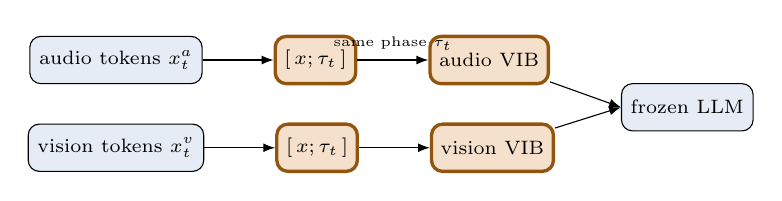
\begin{tikzpicture}[font=\scriptsize,>={Latex[length=1.5mm]},node distance=2mm and 4mm,
  trn/.style={draw,very thick,rounded corners,fill=trn!22,draw=trn!70!black,minimum height=6mm,align=center},
  frzs/.style={draw,rounded corners,fill=frz!12,minimum height=6mm,align=center}]
  \node[frzs] (a) {audio tokens $x^a_t$};
  \node[frzs,below=5mm of a] (v) {vision tokens $x^v_t$};
  \node[trn,right=9mm of a] (ca) {$[\,x;\tau_t\,]$};
  \node[trn,right=9mm of v] (cv) {$[\,x;\tau_t\,]$};
  \node[trn,right=9mm of ca] (ba) {audio VIB};
  \node[trn,right=9mm of cv] (bv) {vision VIB};
  \node[frzs,right=9mm of ba,yshift=-6mm] (llm) {frozen LLM};
  \draw[->] (a)--(ca); \draw[->] (v)--(cv);
  \draw[->] (ca)--node[above]{\tiny same phase $\tau_t$}(ba); \draw[->] (cv)--(bv);
  \draw[->] (ba)--(llm.west); \draw[->] (bv)--(llm.west);
\end{tikzpicture}
\vfill
\begin{itemize}\small
\item Today the bottleneck sees every token \textbf{without its time}. A shared phase $\tau_t$
across both streams makes misalignment \emph{representable}: audio at $t$ and a frame at
$t{+}\Delta$ now differ in their clocks.
\item At 2\,fps the frame grid is $0.5$\,s, so $\pm0.5$\,s is the smallest offset we can honestly ask
about.
\item $W_{\text{out}}$ stays zero-init $\Rightarrow$ still \textbf{identity at start}.
\item[] {\footnotesize\emph{Status: implemented and training; no trained numbers yet.}}
\end{itemize}
\end{frame}

% ================================================================
% ================================================================

\begin{frame}{Ablation: does it matter \emph{where} the bottleneck sits?}
\centering
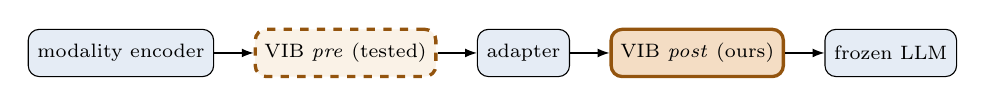
\begin{tikzpicture}[font=\scriptsize,>={Latex[length=1.5mm]},node distance=2mm and 5mm,
  frzs/.style={draw,rounded corners,fill=frz!12,minimum height=6mm,align=center},
  vibs/.style={draw,very thick,rounded corners,fill=trn!25,draw=trn!70!black,minimum height=6mm,align=center},
  vibd/.style={draw,very thick,dashed,rounded corners,fill=trn!10,draw=trn!70!black,minimum height=6mm,align=center}]
  \node[frzs] (enc) {modality encoder};
  \node[vibd,right=of enc] (pre) {VIB \emph{pre} (tested)};
  \node[frzs,right=of pre] (ad) {adapter};
  \node[vibs,right=of ad] (post) {VIB \emph{post} (ours)};
  \node[frzs,right=of post] (llm) {frozen LLM};
  \draw[->] (enc)--(pre); \draw[->] (pre)--(ad); \draw[->] (ad)--(post); \draw[->] (post)--(llm);
\end{tikzpicture}
\vspace{0.6em}
\begin{itemize}\small
\item Supervisor's question: the VIB currently edits the adapter's \textbf{output} (LLM embedding
space). What if it edits the adapter's \textbf{input} (raw encoder features) instead?
\item \textbf{Finding: it does not materially change the outcome.} Both placements land in the same
range on AVHBench.
\item \textbf{Decision: keep post-adapter} --- one attach dimension ($=$ the LLM width) on every
backbone, so the same code runs on Qwen3 / Qwen2.5 / VideoLLaMA2 / MiniCPM-O. Pre-adapter needs a
different width per modality \emph{and} per backbone.
\item[] {\footnotesize\emph{Status: the pre-adapter attach is implemented in this repo
(\texttt{--pre-adapter}); the exact numbers from the earlier run are not in the current results
directory, so no table is shown here.}}
\end{itemize}
\end{frame}

\begin{frame}{What did \emph{not} work --- and what each failure taught}
\centering
\renewcommand{\arraystretch}{1.3}
\scriptsize
\begin{tabular}{l l l}
\toprule
tried & failure & lesson \\
\midrule
na\"ive swap-DPO & collapse to constant ``no'' (PA $0.95\!\to\!0.10$) & metrics can be gamed $\to$ two rails \\
GRPO on easy yes/no items & zero advantage on $\sim$2/3 of steps: no gradient & unanimous rewards teach nothing \\
FiLM's hard gate $g(q)$ & never closed (stayed $>0.4$) & the model preferred \emph{modulation} over routing \\
``vision rewrites 59\%'' claim & overturned by auditing the weights & \textbf{measure, don't assume} \\
LoRA at the same attach points & $+2.8$ vs VIB's $+5.1$; HR drops below base & the \emph{residual form} matters, not capacity \\
\bottomrule
\end{tabular}
\vfill
{\small Half of these became the project's actual content. Negative results are data.}
\end{frame}

\begin{frame}{Reproducibility}
\begin{columns}[T]
\begin{column}{0.52\textwidth}
\textbf{What exists}
\begin{itemize}\footnotesize
\item 4 model wrappers, 5 benchmark runners, 4 training arms, 2 baselines, 3 probes
\item $\sim$10k lines, 23 cluster pipelines, 7 test suites
\item one script per table, one command per figure
\end{itemize}
\end{column}
\begin{column}{0.48\textwidth}
\textbf{What is pinned}
\begin{itemize}\footnotesize
\item frame rate (2\,fps), prompts, answer suffix, decoding
\item checkpoint selection on a disjoint validation half
\item per-item predictions saved $\Rightarrow$ paired tests are recomputable
\end{itemize}
\end{column}
\end{columns}
\vfill
\begin{center}
\setbeamercolor{block body}{bg=blue!6}
\begin{block}{}
\centering\small Every number in this deck is either measured by us (source JSON named in the
source file) or reported by a cited paper. Nothing is extrapolated.
\end{block}
\end{center}
\end{frame}

\begin{frame}{Conclusion}
\begin{itemize}
\item \textbf{Problem}: frozen AV-LLMs over-trust vision; audio evidence loses --- and on the
temporal axis they are at \textbf{chance} (0.495 measured).
\item \textbf{Method}: a $<$0.5\% zero-init variational adapter $+$ audio-swap preference training
$+$ two rails against collapse; a prompt-aware FiLM variant on top.
\item \textbf{Result}: \textbf{$+5.1$ / $+5.8$} AVHBench points, $p<10^{-4}$ paired, capability
preserved on CMM and within noise on MMAU / Video-MME.
\item \textbf{Mechanism}: FiLM is the \emph{only} arm that raises attention to AV tokens
($5.4 \to 7.4\%$); DPO grounds by re-encoding instead.
\item \textbf{Limits}: the gain needs a backbone that already carries audio (null on VideoLLaMA2),
and off-distribution audio reasoning pays a small tax.
\item \textbf{Next}: temporal grounding --- the same engine pointed at \emph{when}, not just
\emph{what}.
\end{itemize}
\vfill
\begin{center}
\setbeamercolor{block body}{bg=blue!6}
\begin{block}{}
\centering\small A tiny adapter, trained without touching the backbone, makes a frozen AV-LLM
listen --- and we can show it is listening, not just scoring higher.
\end{block}
\end{center}
\end{frame}

\begin{frame}{Thank you}
\begin{columns}[T]
\begin{column}{0.58\textwidth}
\textbf{Acknowledgements}
\begin{itemize}\small
\item \fillin{supervisor} and the \fillin{host laboratory} team.
\item Compute: \fillin{ABCI / cluster}, group \fillin{allocation}.
\end{itemize}
\vspace{0.6em}
\textbf{In flight at submission time}
\begin{itemize}\small
\item swap-video and shift-DPO arms; cross-attention arm
\item MiniCPM-O adapter training
\end{itemize}
\end{column}
\begin{column}{0.42\textwidth}
\centering
\vspace{0.4em}
{\Large Questions?}\\[1.2em]
{\footnotesize \color{gray} Souleiman Sbai\\ \fillin{email / contact}}
\end{column}
\end{columns}
\end{frame}

\end{document}
